\begin{figure}[t]
    \centering
    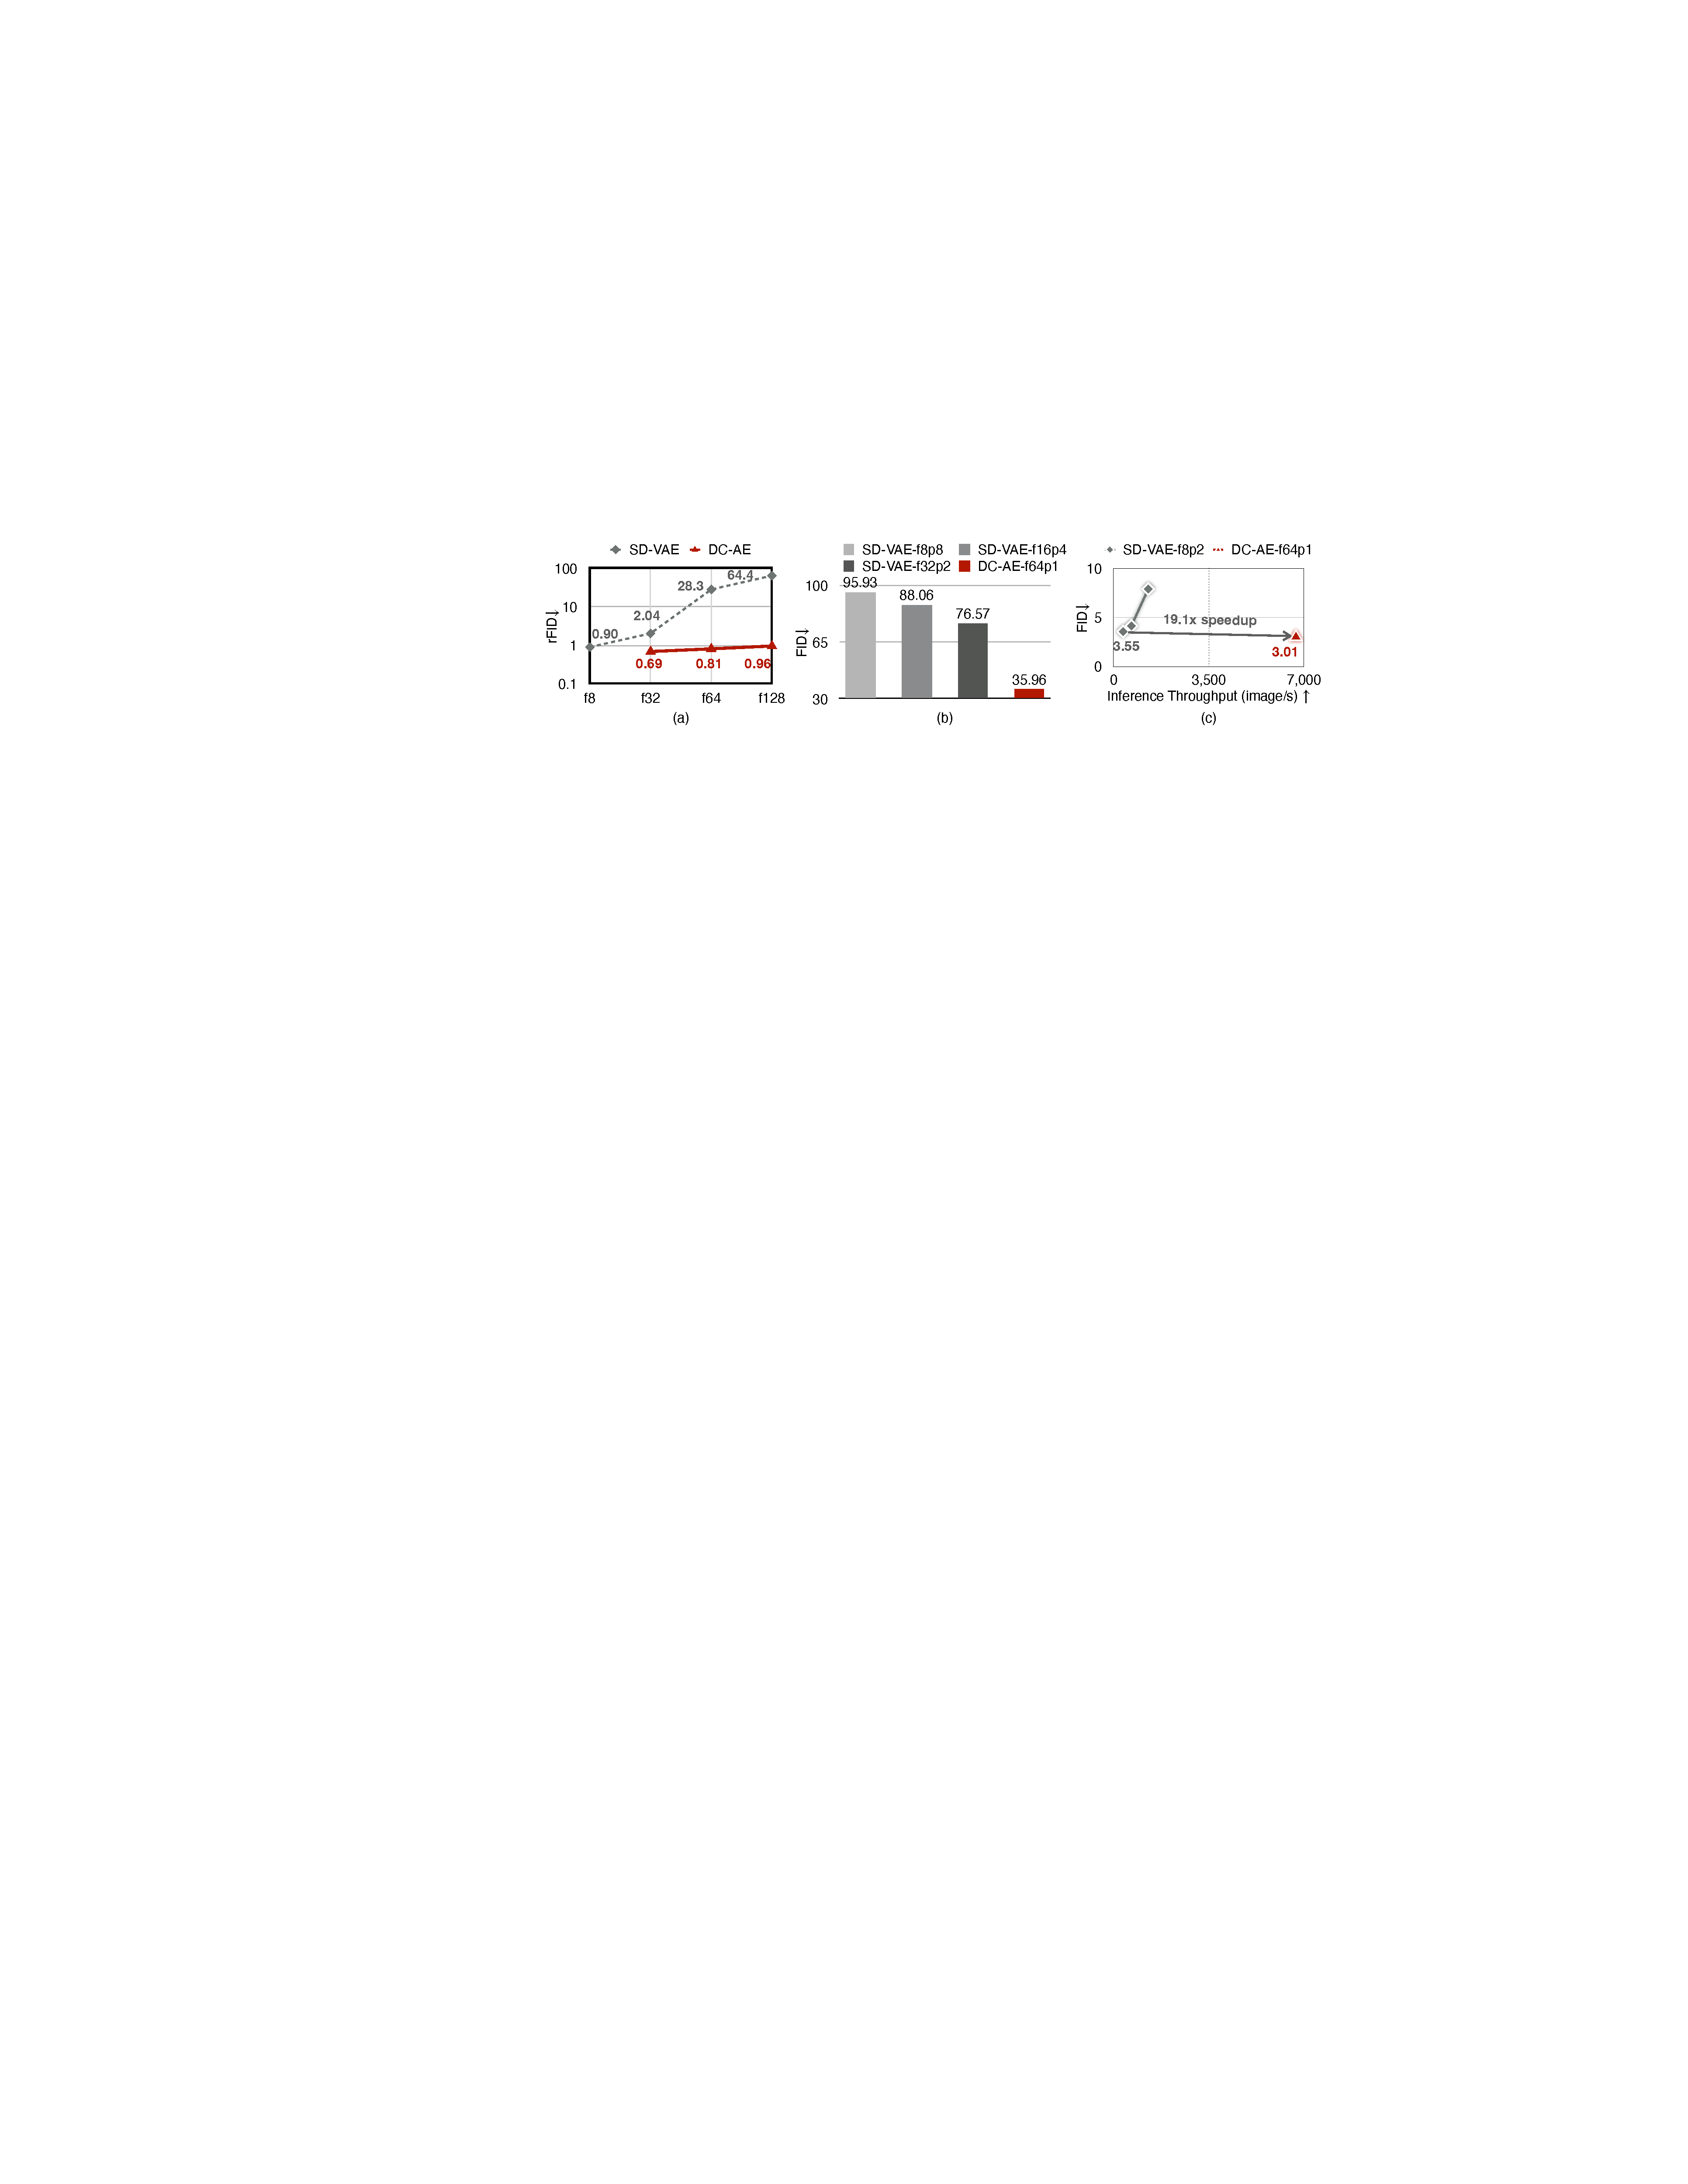
\includegraphics[width=1\linewidth]{figures/src/figure1_results.pdf}
    \vspace{-15pt}
    \caption{\textbf{(a) Image Reconstruction Results on ImageNet 256$\times$256.} f denotes the spatial compression ratio. When the spatial compression ratio increases, SD-VAE has a significant reconstruction accuracy drop (higher rFID) while \modelshort does not have this issue. \textbf{(b) ImageNet 512$\times$512 Image Generation Results on UViT-S with Various Autoencoders.} p denotes the patch size. Shifting the token compression task to the autoencoder enables the diffusion model to focus more on the denoising task, leading to better FID. \textbf{(c) Comparison to SD-VAE-f8 on ImageNet 512$\times$512 with UViT Variants.} \modelshort-f64p1 provides 19.1$\times$ higher inference throughput and 0.54 better ImageNet FID than SD-VAE-f8p2 on UViT-H.}
    \vspace{-10pt}
    \label{fig:figure1_results}
\end{figure}
